\begin{frame}{Boundary Layer Initialization}
    \begin{itemize}
    \item Avoid Instabilities (close to the leading edge)
    \item Avoid velocity ramping
    \item Allows Higher time-step
    \end{itemize}


    \begin{figure}[h]
        \centering          
        \begin{subfigure}[h]{0.45\textwidth}
                 \centering
            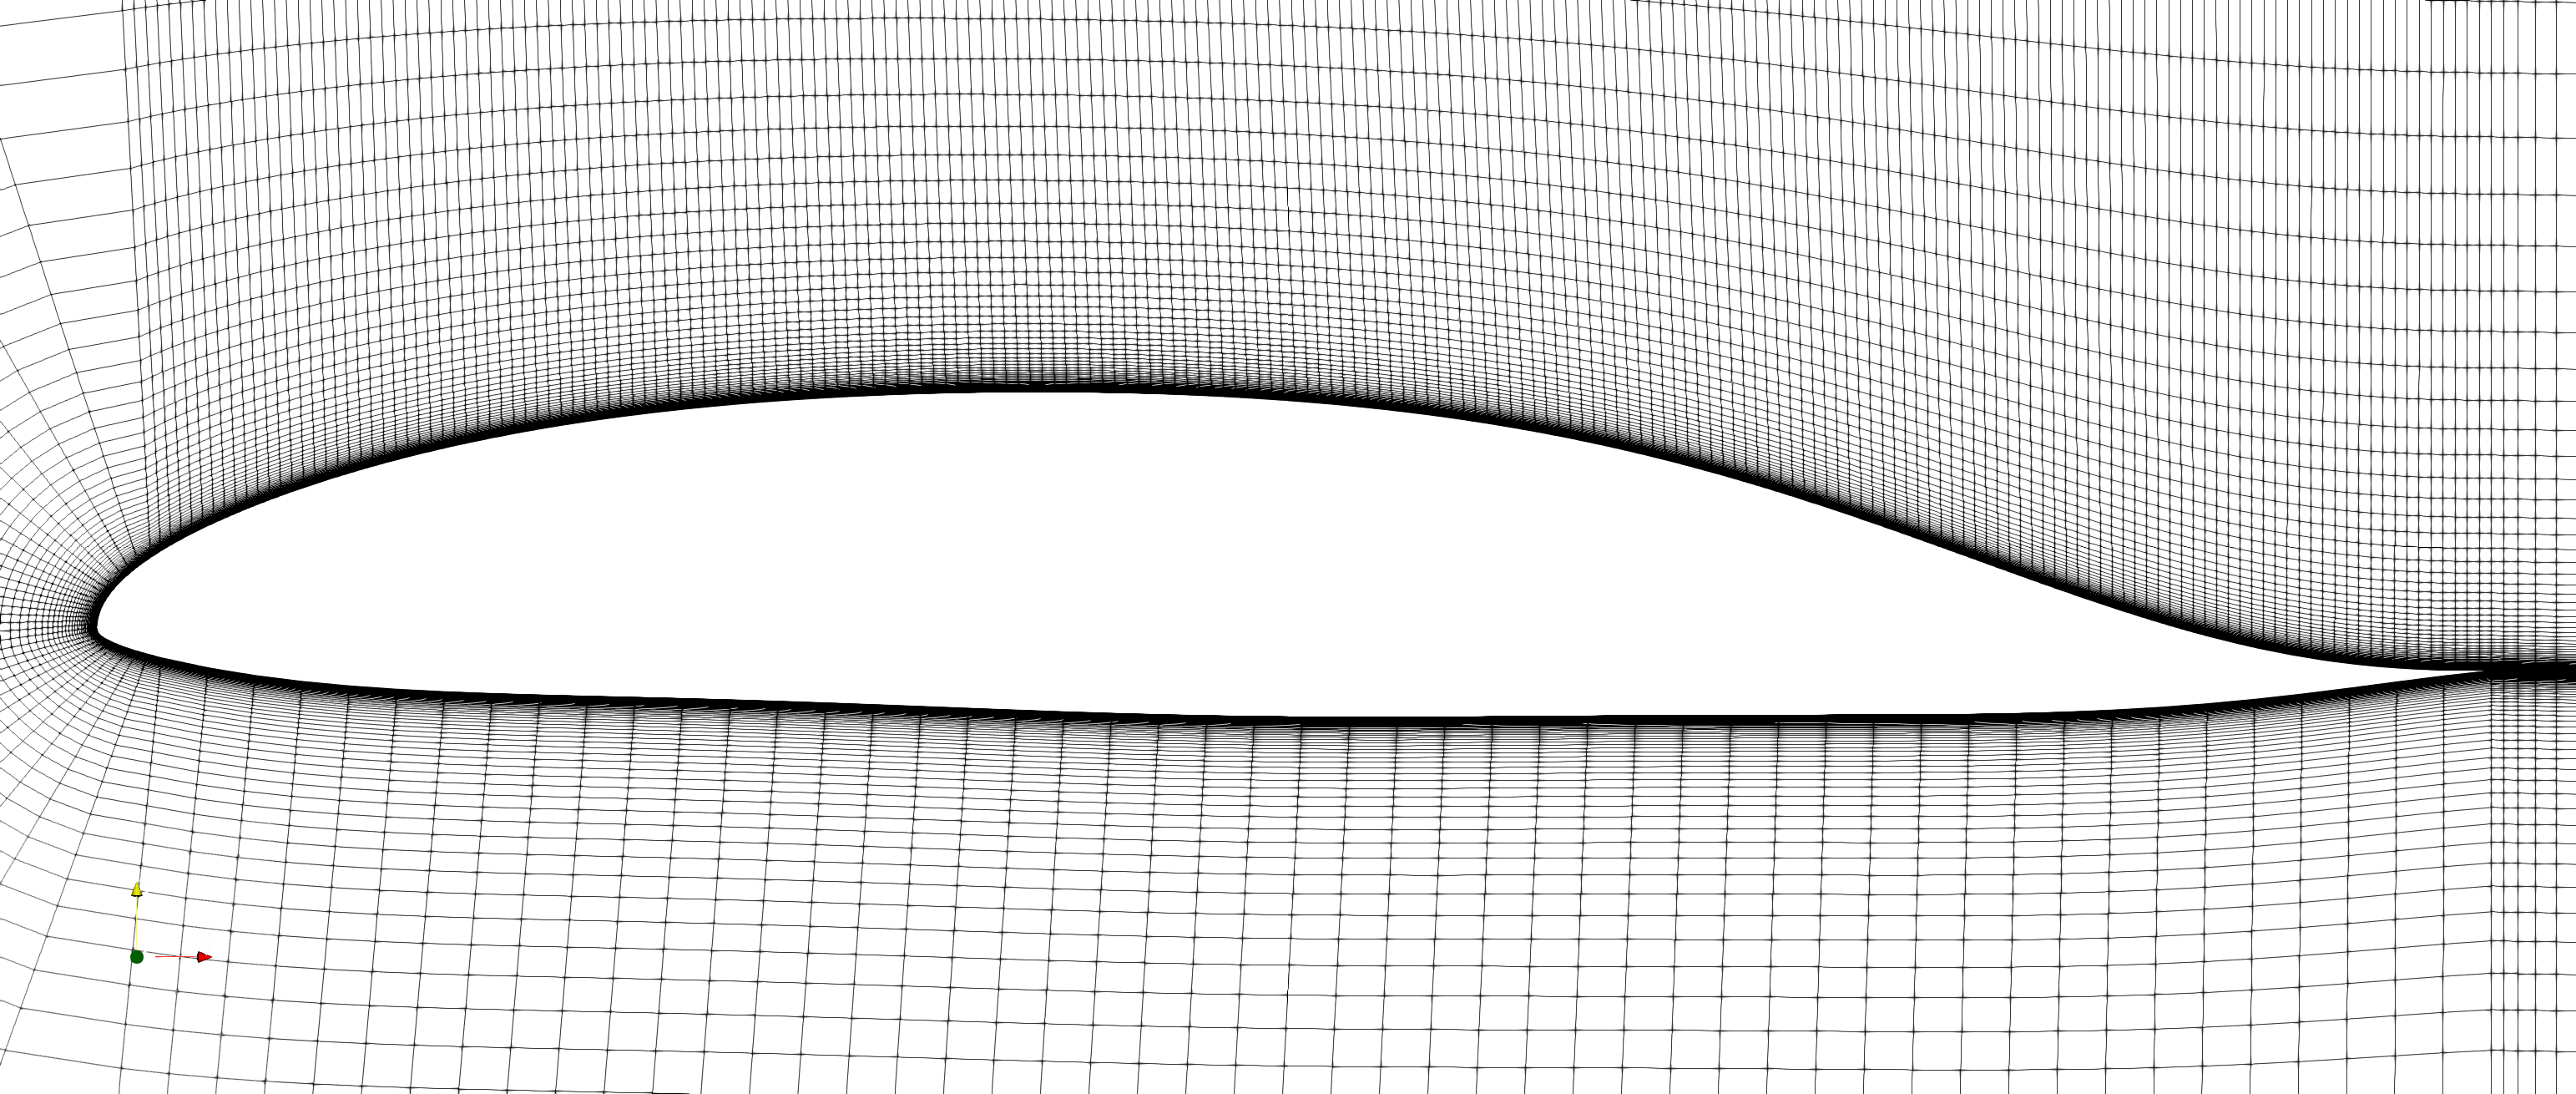
\includegraphics[width=\textwidth]{mesh_du89.png}
       \end{subfigure}
             \hfill
        \begin{subfigure}[h]{0.45\textwidth}
         \centering
            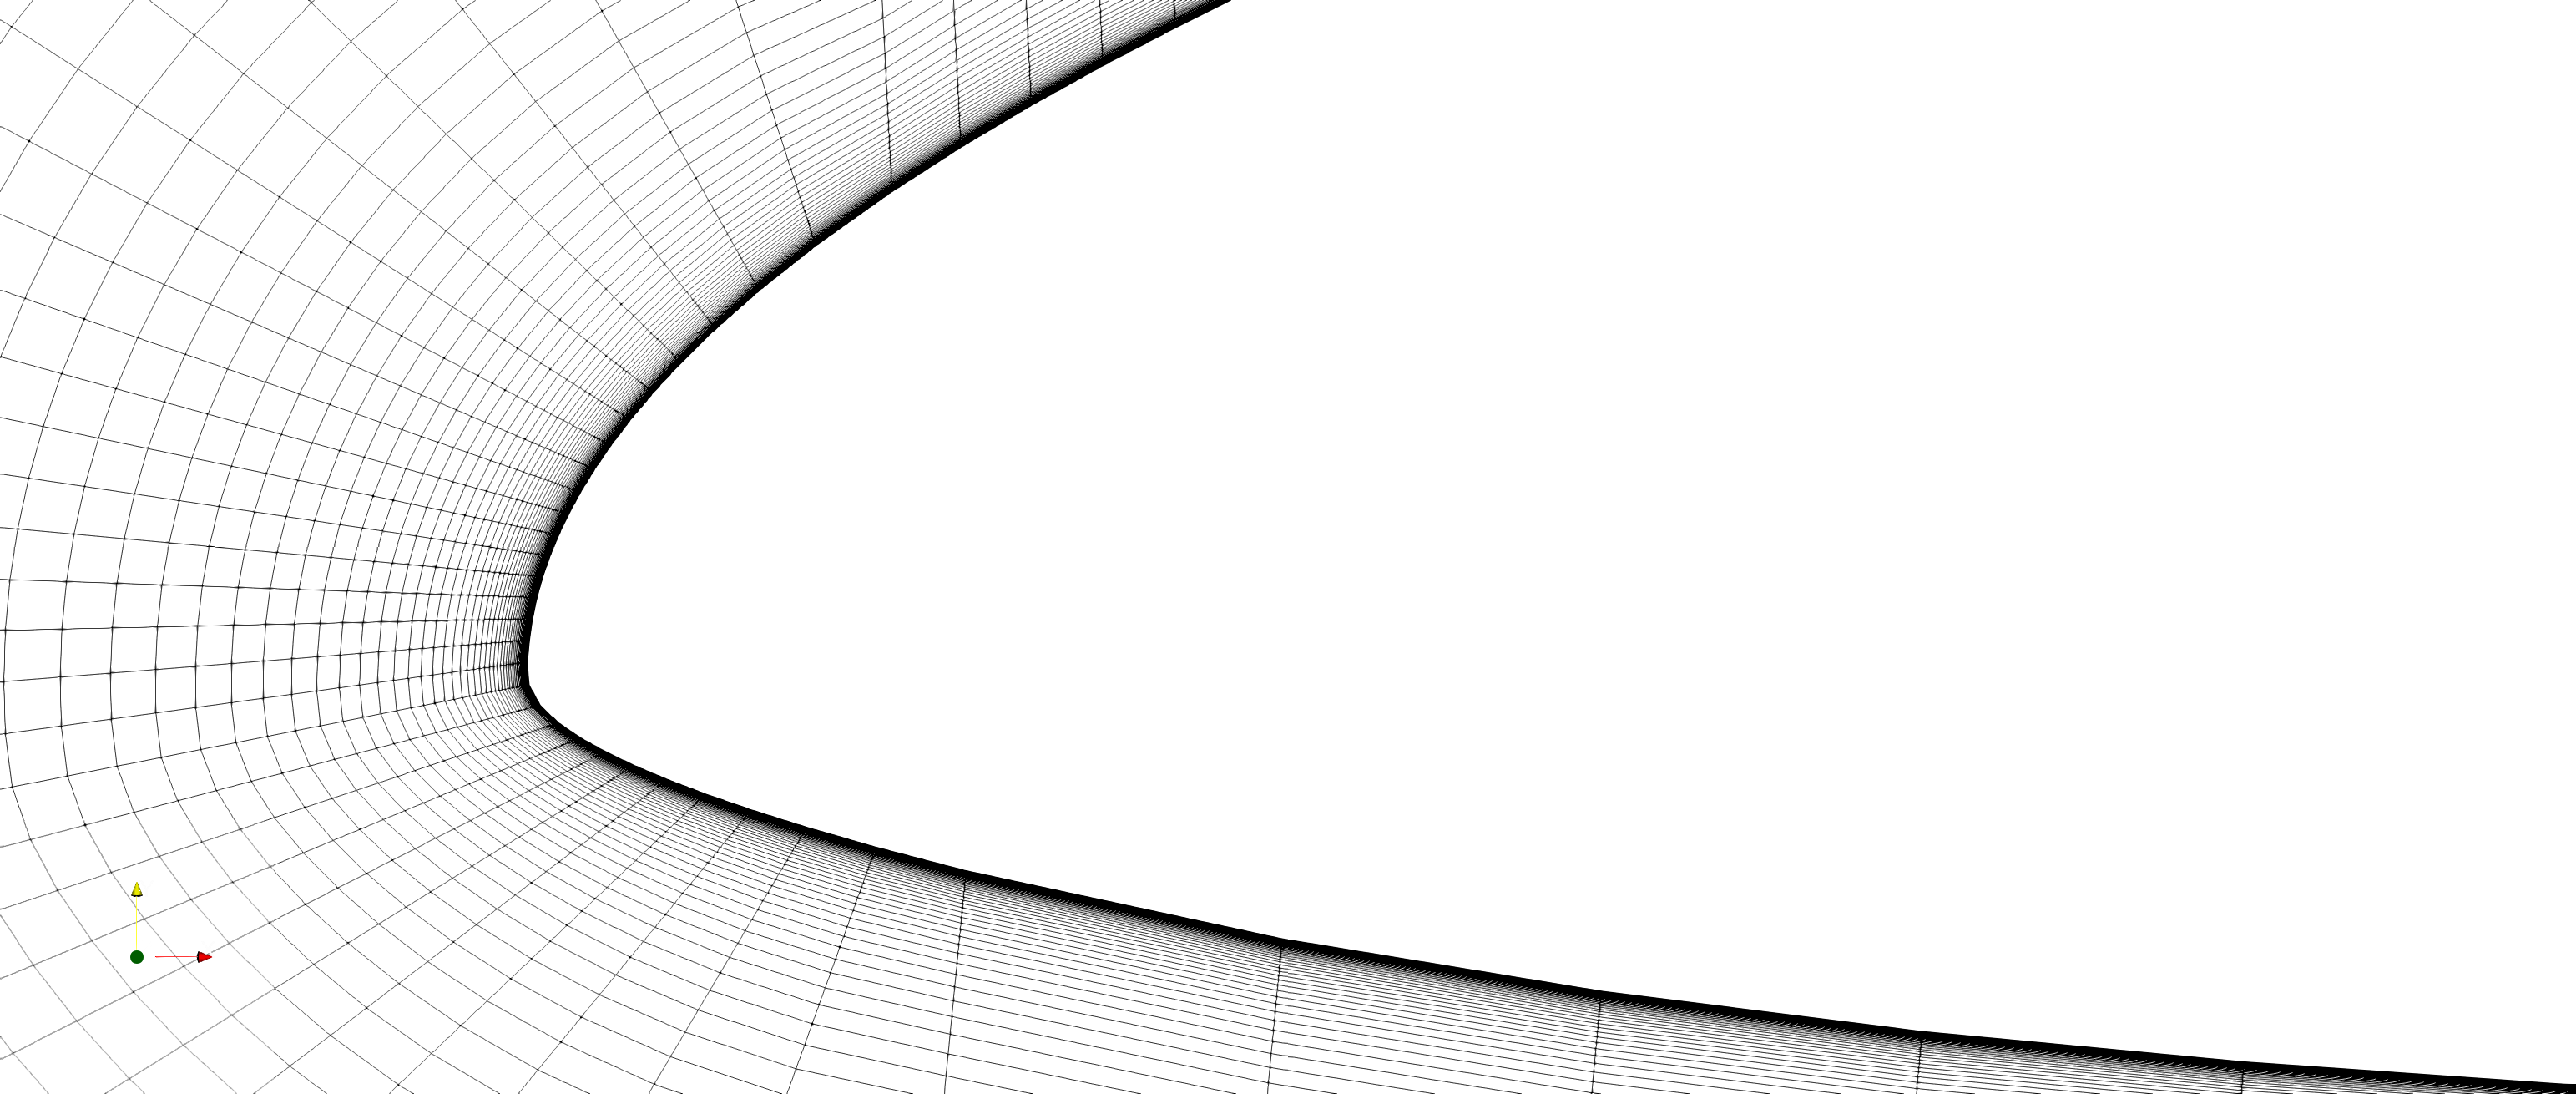
\includegraphics[width=\textwidth]{mesh_du89_le.png}
        \end{subfigure}
        \caption{Mesh DU89}
        \end{figure} 
\end{frame}



\begin{frame}{Find wall-distance}

    Using the function exploited by RANS solvers for the wall distance for computing turbulent parameters but now used to detect the airfoil's contour
    \begin{equation}
    \begin{cases}
        \nabla \cdot (|\nabla u_p|^{p-2} \nabla u_p) = -1 & x\in \Omega\\
        u_p = 0 & x\in \Omega_D
        \end{cases}
        \label{equ:ppoisson}
    \end{equation}
    The true-wall distance is provided by solving the equation for $p\xrightarrow{}\infty$
    Solved using a method that resembles Picard's
    \end{frame}
    

    \begin{frame}{Find wall-distance}
    \begin{equation}
        v_p = -|\nabla u_p|^{p-1} + \bigg ( \dfrac{p}{p-1}u_p +  |\nabla u_p|^{p}\bigg ) ^{\dfrac{p}{p-1}}
        \label{equ:vpoisson}
    \end{equation}
    \begin{enumerate}
        \item It starts solving the equation for p=2
        \item \begin{equation}
            \int \bigg (\nabla (v) \cdot (\nabla u_{hp}) \bigg )d\Omega = \int \bigg( 1\cdot v \bigg )d\Omega
        \end{equation}
        \item It solves the linearized equation, which becomes \eqref{equ:ppoisson-fem2}. In this case solving for p=3 the $\tilde{u}$ is $uh_2$
          \begin{equation}
            \int \bigg (\nabla (v) \cdot (|\nabla \tilde{u}|^{p-2} \nabla u) \bigg )d\Omega = \int \bigg( 1\cdot v \bigg )d\Omega
            \label{equ:ppoisson-fem2}
        \end{equation}
        \item It is not possible to iterate step 3 for p > 3, the solution becomes unstable. It introduces the relaxation coefficient $\gamma = 0.5$ and it starts an internal cycle.
    \end{enumerate}
    \end{frame}

    \begin{frame}{Boundary Layer Initialization}
    The velocity in the $x$ direction in the region identified can be with a simple cubic function \eqref{equ:bl-cubic-init} where $dn = d/\delta_{99}$, $d$ is the minimum distance to the airfoil, $u_\infty$ is the free-stream flow speed.
    \begin{equation}
        f(dn) = 
        \begin{cases}
            u_\infty & dn>1\\
            ( -dn^2+2\cdot dn )\cdot u_\infty &  dn<1
        \end{cases}
        \label{equ:bl-cubic-init}
    \end{equation}
     The boundary layer function has been obtained by fixing the following boundary conditions:
    \begin{itemize}
        \item Continuity with the external flow, $f(1)=1$ 
        \item Smooth transition between boundary layer and external flow, $f'(1)=0$ 
        \item Non-slip condition at the wall, $f(0)=0$
    \end{itemize}
    \end{frame}
    
    \begin{frame}{Boundary Layer Initialization}
    It results in a low-speed zone close to the airfoil, avoiding high speed in really small cells useful for capturing the boundary layer.
    \begin{figure}
             \centering
             \includegraphics[width=0.65\textwidth]{WallDistanceDU89.png}
             \caption{Boundary Layer Initialization}
             \label{fig:wall-distance-init}
    \end{figure} 
    \end{frame}
    